\author{Bautrelle Fotso}
\graphicspath{ {./src/chapters/developer/media/} }

\section{Networks}
In the previous section, many types of datasets and their characteristics have been presented. 
However, the use of datasets is not sufficient to perform the Optical Character Recognition (OCR). 
These datasets have to be applied to different networks which learn from them. 
The goal is to obtain a model with the best accuracy for each OCR case handled in this project, namely: number, text and text without number.
This process is called deep learning. 

\noindent
Accordingly, deep learning can be defined as a subset of machine learning to preprocess data in artificial 
intelligence. For this task, it imitates the working of the human nervous system.  
Like machine learning, deep learning has the particularity of learning in an unsupervised way from unstructured datasets.  
Learning in an unsupervised way means that, the network receives inputs without outputs. 
During the training, the network must decide itself which output is corresponding to the input received.(\cite{[1]}, p.6)
Deep learning is a term to describe deep neural networks and their functionalities. 
The word "deep" specifies that the network always contains more than one intermediate layer.(\cite{[1]}, p.8) \hfill \break

\noindent
Three types of deep neural network have been used in this project and are described in this section. These are:

\begin{itemize}
    \item Deep Feedforward Neural Network(DFFNN)
    \item Convolutional Neural Network(CNN)
    \item Recurrent Neural Network(RNN).

\end{itemize}


\subsection{Deep Feedforward Neural Network(DFFNN)}
The Deep Feedforward Neural Network, also called Multi-Layer Perceptron(MLP), is a network composed of an input layer,
at least two hidden layers and one output layer. 
In this network, each neuron in the previous layer is connected with all neurons of the next layer to form a fully connected layer. 
Additionally, the connection between two neurons in the network has a certain amplitude called weight. (\cite{[1]}, p.4) 

\noindent
The EMNIST-letters and the MNIST datasets have been applied on this network for the main reason that, they are compatible together. \hfill \break

\noindent
The picture (\ref{Abb:feed_forward}) below illustrates a general model of DFFNN.

\begin{figure}[htb]
	\centering
	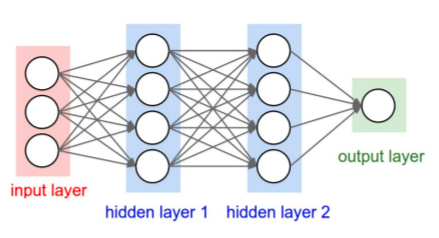
\includegraphics[height=0.2\textheight]{simple_FFNN}
	\caption[Deep Feedforward Neural Network]{Deep Feedforward Neural Network (\cite{[3]}, p.1)}\label{Abb:feed_forward}
\end{figure}

%\newpage
\noindent
This is just a general overview of DFFNN, however, a specific network needs to be built accordingly to 
the requirements of this project. \hfill \break

\subsubsection{Building the Deep Feedforward Neural Network}
An example of DFFNN built on MNIST dataset is presented in the figure(\ref{Abb:build_feed_forward}).

\begin{figure}[htb]
	\centering
	\includegraphics[width=1.0\textwidth]{ffnn}
	\caption[Build Deep Feedforward Neural Network]{Building the Deep Feedforward Neural Network on MNIST dataset} \label{Abb:build_feed_forward}
\end{figure}

\noindent
A sniped code of a built DFFNN an its abstract representation can be seen respectively on the left  
and on the right side of the picture(\ref{Abb:build_feed_forward}). 
The architecture used to build this network is the sequential mode of the keras library. 
It is always appplied when the network takes only one input and one output layer. 
This sequential mode specifies to keras that the output of each layer added should be used as input in the next layer. 
The function for adding each layer to the network is \emph{add()}. 
The first layer of the network takes a vector as input. 
But the dataset images used to train the network have the shape of 28x28 pixels (28 for the height x 28 for the width of the image). 
Each image is transformed to a vector of 784 pixels with the function \emph{Flatten()}, which receives as parameter 
the shape of the image to be converted. This shape can be a tuple of (28, 28) or a triplet of (1, 28, 28). 
The "1" in the triplet just specifies the number of image with the shape 28x28 pixels. 
These notations are equivalent because the input layer takes only one image at the time. 
The two hidden layers are also added with 512 neurons each. 
With the function \emph{Dense()}, a full connection is created between neurons of the previous layer and the next layer. 
The activation function \emph{"relu"}(Rectified Linear Unit) is a linear function used to remove negative activations.
It is the most used activation in deep learning(\cite{[1]}, p.12). 
An activation is the occupancy rate that an image takes on each of its pixels. 
This will be more explained in the training part. 
On the last layer the number of neurons is determined by the number of classes available in the used dataset. 
The output contains ten neurons ranging from 0 to 9 corresponding to the ten classes of MNIST. 
The activation function \emph{"softmax"} maps the prediction vector obtained in the output layer to a probability distribution.
In this case, the prediction vector has ten indices, whose values are represented as probabilities in the range [0,1]. 
At the end, all added layers are put together using the function \emph{compile()}. 
The network uses \emph{"adam"} optimizer responsible to update weights between neurons after a forward pass. 
By the forward pass, activations are diffused only forward from the input layer, through the hidden layers to the output 
layer and consequently has no loops.
Updating the weights means adjusting it so that the difference between the real values and the values predicted by 
the trained model will be minimized. 
This difference is called \emph{"loss"} and is calculated using the loss function \emph{sparse\_categorical\_cross\_entropy}. 
This type of loss function is especially applied on this network because the labels of the MNIST dataset have not been one-hot-encoded. 
One hot encoding transforms a label, which is represented as an integer, to a binary value represented as a vector. 
Using this loss function also help to save time as well as computation because it simply takes a single integer rather than a whole vector. 
The chosen metric is the accuracy, which indicates how good the prediction rate on training data is, after each forward pass. (\cite{[4]})

The network training is then started by the function \emph{fit()} called on the built network(the variable model). 

\noindent
In the following part, the training of the model  and the role of each parameter used in the function \emph{fit()} will be explained. 


\subsubsection{Training the Deep Feedforward Neural Network}
The next step, after building a network, is to train data on it to obtain a model suitable for prediction.
The following picture presents the training process of the DFFNN on the MNIST dataset.

\begin{figure}[htb]
	\centering
	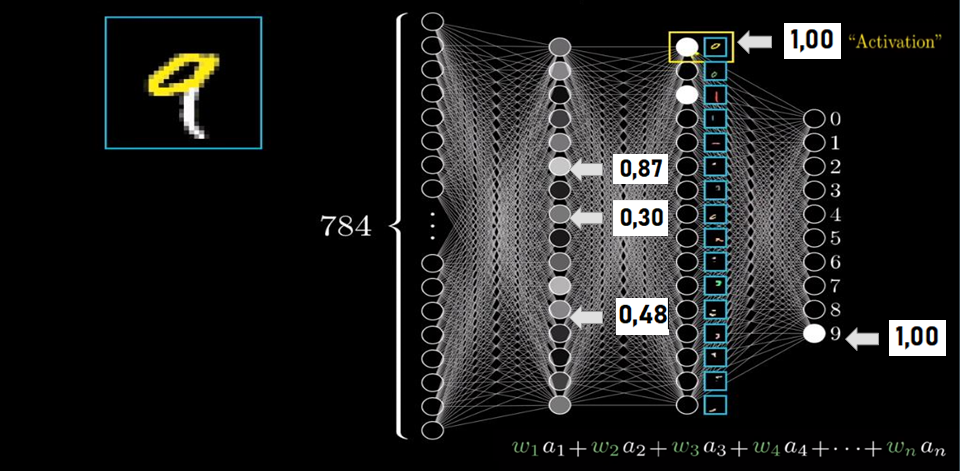
\includegraphics[width=1.0\textwidth]{train_cnn}
	\caption[Train Deep Feedforward Neural Network]{Training the Deep Feedforward Neural Network on MNIST dataset \cite{[12]}} \label{Abb:train_cnn}
\end{figure}
The MNIST dataset, namely the train and the test set have to be first loaded from the \emph{Keras.dataset.mnist} library. 
After loading the dataset, 
the train and the test set images are rescaled to be sure that the required size is kept. 
Afterward, each image pixel is downscaled from [0 255] to [0 1], to maintain a general pixel value distribution on the entire dataset 
and avoid working with big decimal values. 
For a better training of the dataset, the network uses mini-batches of the MNIST training data instead of the entire dataset at once. 
The actual training is started using the function model.fit() as mentioned above. 
At the end of each epoch, the network will be evaluated on the test data, which have not been trained.
An epoch describes an unique passage of the entire MNIST dataset through the network. 
After the dataset images have been normalized and reshaped, the built network then receives a digit image of 28x28 pixels as input. 
This image is flattened to a vector of 784 pixels. 
Each of these pixels represents a neuron in the input layers. Each neuron holds a specific number
in the interval of 0 to 1 due to the previous normalization (division of each pixel value by 255). 
The value contained in these neurons represents the value of the corresponding 
pixel, which is called \emph{activation}. When a neuron is brighter, the activation is high and tends towards 1. 
Otherwise, the activation is low and tends towards 0. 
One important thing to notice on training networks is that, the activation value of the previous layer is always used to determine 
the one of the next layer. This is realized by doing a particular calculation. 
An example of the computation with some results is shown on the figure(\ref{Abb:train_cnn}). The activation values 
are not real, but it has been used for illustration purpose. 
For this example, there are two neurons on the third layer with the highest activation 1. They have the form of a "zero" and a 
"dash", whose combination gives on the fourth layer the correct predicted answer nine(9).
After each forward pass from a layer to the other, the weights muss be updated before a next pass. 
This loss value obtained from the function \emph{sparse\_categorical\_cross\_entropy} is sent back through each layer and the 
optimizer(adam) bases its computation on this error rate. This helps to update 
the weights accordingly to the error rate of each of this weights, in order to minimize the error by the next forward pass. 


\subsubsection{Results and interpretation}
The prediction results of the model obtained by training DFFNN on the MNIST dataset are in the figure(\ref{Abb:mnist_metrics}). 

\begin{figure}[htb]
	\centering
	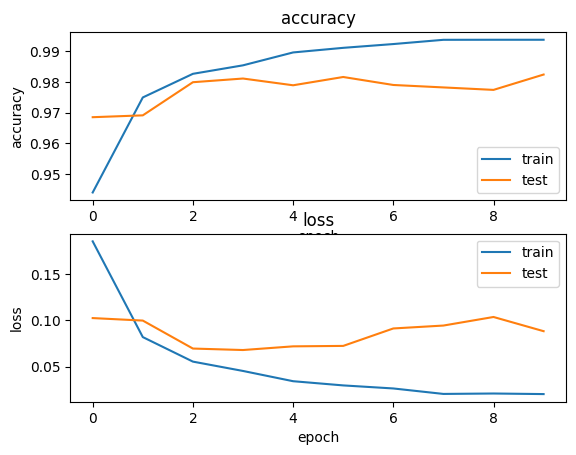
\includegraphics[width=0.4\textwidth]{MNIST_metrics}
	\caption[Results of DFFNN model on MNIST]{Loss and Accuracy from DFFNN model on MNIST train and test set} \label{Abb:mnist_metrics}
\end{figure}

The model prediction results of the MNIST training and test set are obtained during a defined number of epochs.
It is observable that, the training set has a higher accuracy and a lower loss value
than the test set.
This can be due to the fact that the training set is the one applied on the network during the training. 
However, the error rate by the test set differs very little from the one by the training set.
It means that, the probability to correctly predict a new image is also high, although the image have not 
been trained on the network before. 


\subsection{Convolutional Neural Network (CNN)}
Convolutional Neural Network is a type of neural network which uses a particular processing for recognizing images. 
CNN is basically used for image analysis. (\cite{[6]}, p.3)
They are three types of CNN: 

\begin{itemize}
    \item One dimensional CNN
    \item two dimensional CNN
    \item three dimensional CNN.
  \end{itemize}

One dimensional CNN takes one dimensional vectors as input. 
It is also applied for digits recognition like DFFNN. The two other types of CNN use a matrix as input(2D or 3D matrices according to the type of CNN).
CNN is an excellent network for object recognition, behavior recognition, natural language processing and more. 
The CNN used in this project is the 2D-CNN. (\cite{[1]}, p.16)

The figure(\ref{Abb:schema_cnn}) presents a schematic diagramm of this network type.
\begin{figure}[htb]
	\centering
	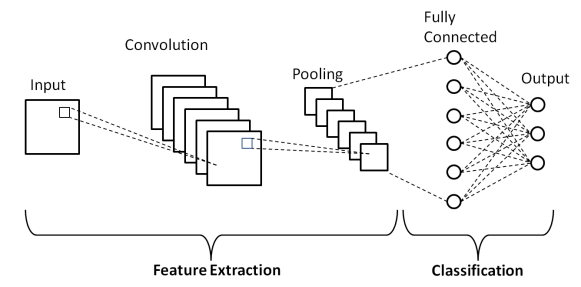
\includegraphics[scale=0.6]{schema_cnn}
	\caption[Convolutional Neural Network]{General view of a Convolutional Neural Network (\cite{[14]})} \label{Abb:schema_cnn}
\end{figure}

As seen in figure(\ref{Abb:schema_cnn}) a CNN generally contains an input layer, a convolutional layer and  a pooling layer. They help not only to 
analyze an entire image in pieces but also extract its features for a better recognition; this makes the difference CNNs and DFFNNs. 
The second part of this network is made up of a fully connected layer for predictions of images. At the end of the prediction process the 
results are then forwarded to the output layer.
Figure(\ref{Abb:schema_cnn}) has been chosen for illustrative reasons. 
For better performance, a CNN must have more than one of each layer mentioned above. (\cite{[1]}, p.16)

\subsubsection{Building the Convolutional Neural Net}
This part explains how the 2D-CNN was constructed appropriately to the requirements of the data to be applied on it. 
Three datasets have been used on this network, namely the EMNIST-balanced, EMNIST-byMerge and EMNIST-digits datasets. 
The following application example is based on the building of the 2D-CNN model to recognize the EMNIST-Balanced dataset.

\begin{figure}[htb]
	\centering
	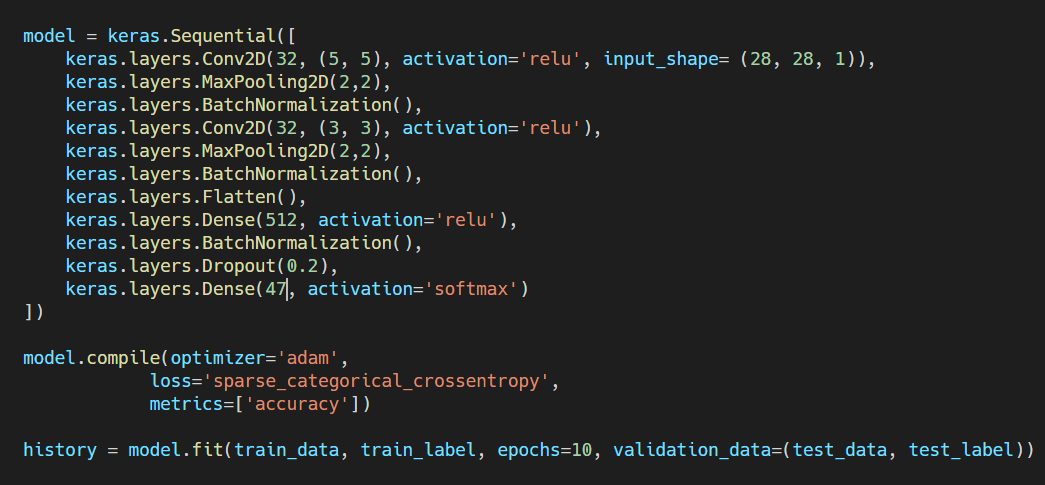
\includegraphics[width=1.0\textwidth]{build_cnn}
	\caption[Building Convolutional Neural Network]{Building the Convolutional Neural Network on EMNIST-Balanced dataset} \label{Abb:build_cnn}
\end{figure}

\noindent
As shown in the figure above, The 2D-CNN is also built using a sequential architecture. 
It is constituated of some components, similar to those in the DFFNN. 
As explained above, the 2D-CNN takes a 2D-matrix as input parameter. In this case either an image of the  
size (28, 28, 1) or the size (1, 28, 28, 1) can be used.
The last value "1" of each size specifies the channel of the image. The channel 1 describes grayscaled images and the channel 3 color images.
Like DFFNN, each input layer recognizes automatically the value "1" of each size, as first element of the input shape.
The first layer is the \emph{2D-convolutional layer}. On this layer 32 filters are defined with a size of 5x5 each.
Each of these filters are used to filter each area of the image. 
Activation functions are similar to those described in the DFFNN. 
The next layer is the pooling layer where the max pooling operation is performed. The \emph{Max pooling layer} is used to downstream 
images obtained from the convolution step, done in the first layer. 
It is used to speed up the processing of the image. 
The \emph{BatchNormalization} is the following layer where the downsampled images obtained from the \emph{Max Pooling layer} are normalized. 
The build process of this three layers is repeated once more to form the next three layers. 
The only difference is the fact that the 32 filters used on the second 2D-convolutional layer has a size of 3x3. 
The \emph{Flatten} layer converts the obtained feature images to a vector in order to make it ready to be used as input in the fully connected 
layer. 
By adding of the \emph{Dropout layer}, 20\% of the neurons in the network will be randomly deactivated during the forward pass on the network.
The weights updating is not applied on dropped out neurons during the backward pass. 
By the Backward pass, information about the difference between the real and the predicted value (loss) are sent back to neurons. 
During the dropout, the remaining neurons have to step in, take the role of the ignored neurons in order to 
handle the representation required to do the prediction. 
This technique avoids the neurons to be dependent from each other and from its context.  
Furthermore, the network will not just memorize the training data but is able to 
realize better generalizations and is more flexible to predict any data. 
This problem of memorizing the training data is called overfitting and the general solution is to implement a 
dropout layer using the activation function \emph{softmax}.  
The Results in the output layer are distributed among 47 neurons because the EMNIST-Letters has 47 classes.


\subsubsection{Training the Convolutional Neural Network}

\begin{figure}[htb]
	\centering
	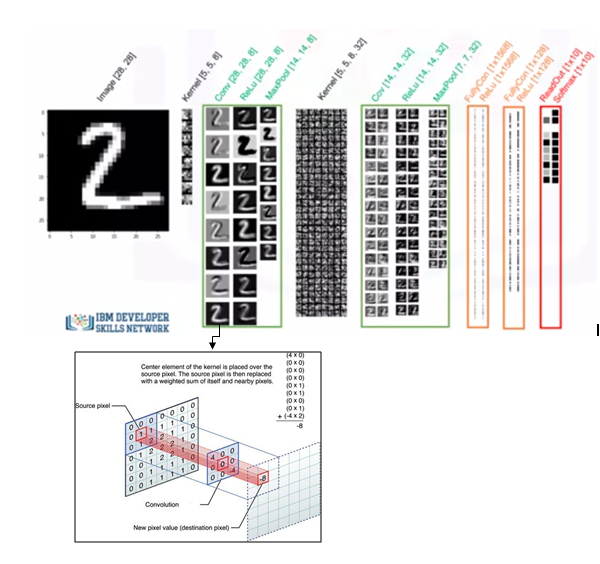
\includegraphics[width=0.8\textwidth]{conv2}
	\caption[Convolutional Neural Network]{Trainings process of the CNN (\cite{[5]})} \label{Abb:cnn_process}
\end{figure}

The upper part of the figure(\ref{Abb:cnn_process}) shows each step of the training on CNN, regardless on whether the CNN is 
a 1D or 2D-CNN because both have almost the same process. 
The only difference is the shape of the input image used for the training. 
Firstly, the image is loaded into the convolutional layer of the CNN. 
In this layer the convolution of the image is performed with each of the 5x5 filter(conv). 
These filters are randomly initialized so that, each of them recognizes specific features of the image such as edges and curves. 
The bottom part of the figure(\ref{Abb:cnn_process}) illustrates how the convolution of an image works.
It is an element-wise multiplication of image pixels with a filter to detect specific features.
The resulting image after the convolution with one filter is called the feature map.
Accordingly,there are 8 feature maps in the first column(conv) of the third picture in figure(\ref{Abb:cnn_process}). 
The feature map can contain negative values. 
The relu activation function is then used to set all negative values to zero, in order to have only positive 
activations in the feature map.
This feature maps are then forwarded to the pooling layer which uses the \emph{maxpool} method. 
The maxpool method itself modifiies the image size by reducing the number of overall parameters in the image. 
As illustrated in the third column of the third picture in figure(\ref{Abb:cnn_process}), the size of the eigth images has reduced to 14x14 pixels. 
In the second 2D-convolutional layer, 32 filters have been used for the convolution. 
The previous steps are repeated again up to the last pooling layer, which has reduced the size of the 32 images (obtained 
after the convolution) to 7x7 pixels. 
The process performed from the first convolutional layer up to the last maxpooling layer is called \emph{feature learning and extraction process}. 
The output of the pooling layers are then flattened and connected to the dense layers. 
After the images have been flattened, the prediction happens similarly to the process in the DFFNN and is called \emph{classification process}. \hfill \break

\subsubsection{Results and interpretation}
The figure(\ref{Abb:emnist_balaced_metrics}) presents the results obtained by the training of CNN on the 
EMNIST-balanced dataset after a defined number of epoch.
It is remarkable that, the training set has a lower loss value than the test set.
This can also be due to the fact that the training set is the one applied on the network during the training. 
However the test data has a model accuracy closed to 90 percent.  
This accuracy describes the performance of the model on data which have not be trained on it.
Through this results, it can be prognosticated that the model is able to correctly predict any character image
with an accuracy of more than 80 percent. 

\begin{figure}[htb]
	\centering
	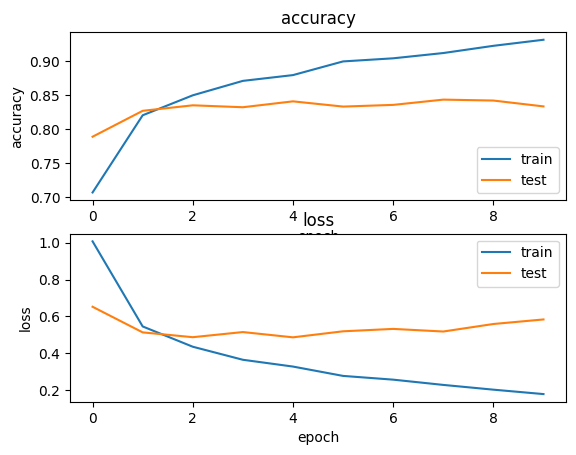
\includegraphics[width=0.4\textwidth]{EMNIST-balanced_metrics}
	\caption[Results of DFFNN training on MNIST]{Loss and Accuracy rates on EMNIST\_balanced got from the 2D-CNN model} \label{Abb:emnist_balaced_metrics}
\end{figure}



\subsection{Recurent Neural Network(RNN)}
The Recurrent Neural Network is a Network, which has been designed for the analysis of sequential data such as 
videos and speechs. 
The particularity of the RNN is that, the information are not only sent forward but also backward 
through the network; this means, the RNNs have loops and also self-feedback loops.
Additionally RNNs have a short memory. 

The figure(\ref{Abb:schema_rnn}) shows a general model on how the RNN is representated.

\begin{figure}[htb]
	\centering
	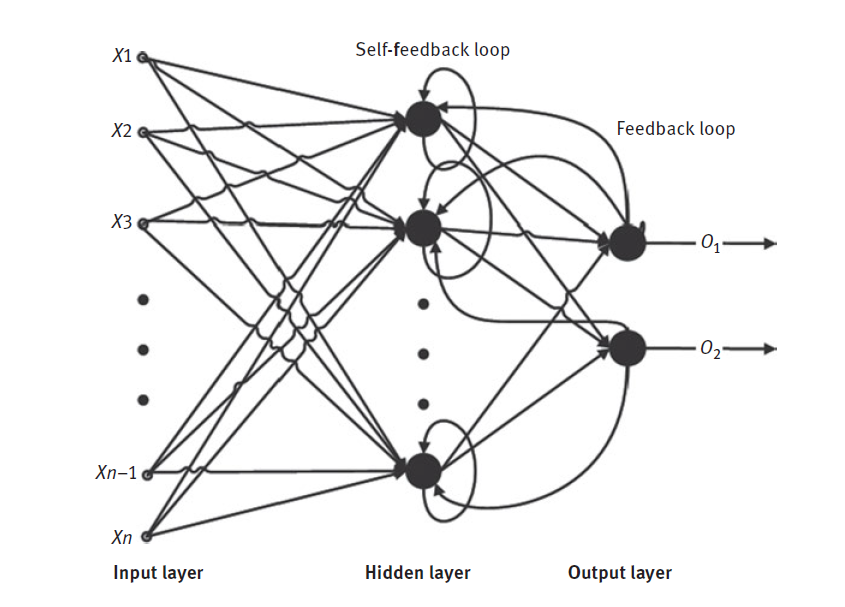
\includegraphics[height=0.3\textheight]{rnn}
	\caption[Schema Recurrent Neural Network]{Representation of the Recurrent Neural Network (\cite{[1]})} \label{Abb:schema_rnn}
\end{figure}

\noindent
The capacity to loop over the layers while training, gives the possibility to get the activation of the next layer 
by computing the current activation (got at the time \emph{t}) with the activation of the previous 
layer (got at the time \emph{t-1}).
This example can be taken as illustration to this concept: when the network is provided with the input "HELLO", the RNN still knows 
by reaching the character "E", that "H" is the character trained before.
This helps especially on sequential data like speechs because each words pronounced have to be saved and not 
immediately thrown away after working on it.
This is not possible by DFFNN and CNN because they have no memory. It is the reason why RNNs have became the state-of-art in natural 
language processing(handwriting, speech, etc.).(\cite{[6]}, p.2)
The main type of the RNN is the Long-short Term Memory (LSTM) because it does not conserves its memory only for a 
short moment but for a long period of time. 
LSTM memory has a read and write function as the one of a computer, with the only difference that 
its memory is analog and not digital. (\cite{[7]})

\noindent
A custom model was not built for this network type. But a tool called \emph{Tesseract-ocr engine}(\cite{[11]}) (which already contains 
the built LSTM), was used. 
Developped from Hewlett Packard betweeen 1984 and 1994 and later taken over from Google(2006), tesseract-ocr 
is an open source for the extraction of texts from images. 
It has a considerable quantity of models for recognition, available in about two hundred different languages. 
Despite the fact that tesseract excellently performs the recognition of printed texts, it is inconsistent by the 
prediction on handwritten texts. 
Nevertheless, tesseract can learn to recognize handwriting, when a custom dataset is built and trained on it. 
This is the reason why the SWTP-AI dataset previously presented has been created.
In the following, the general trainings process of tesseract will be explained.

\subsubsection{Use tesseract to generate a model for text recognition}

\begin{itemize} \bfseries
	\item Installation of dependecies
\end{itemize}
Firstly tesseract-ocr was installed on linux operating system to execute the training process from the command line. 
Then the JTessboxeditor was also installed but this time on windows for the labelling of the data. 
The labelling and the training could happen directly from the JTessBoxEditor because it has integrated functionalities 
to perform both tasks and therefore generate new fonts (models) for tesseract.
But the goal was first of all to learn and understand step by step, how this training works in the background; reason why it has 
been done on Linux kernel.
Since python is used on this project, there is a need to have a module which can be connected with tesseract on local system, 
in order to use some functions on python for predictions with tesseract. 
This module name is \emph{pytesseract}. (\cite{[9]}, \cite{[8]})
The installation of tesseract and pytesseract with all necessary packages can be followed here(\cite{[9]})

\begin{itemize} \bfseries
	\item Labelling handwritten characters for the training
\end{itemize}
About 15 full and long texts have been written from differents persons to have a diversity and a flexibility when using the new model.
When each character of those texts has to be labelled from hand it would have taken too much time. 
Therefore, this step was taken off from JTessBoxEditor.
The labelling consists on correcting wrong characters and box coordinates.

An Example of this can be found on in the figure below.

\begin{figure}[htb]
	\centering
	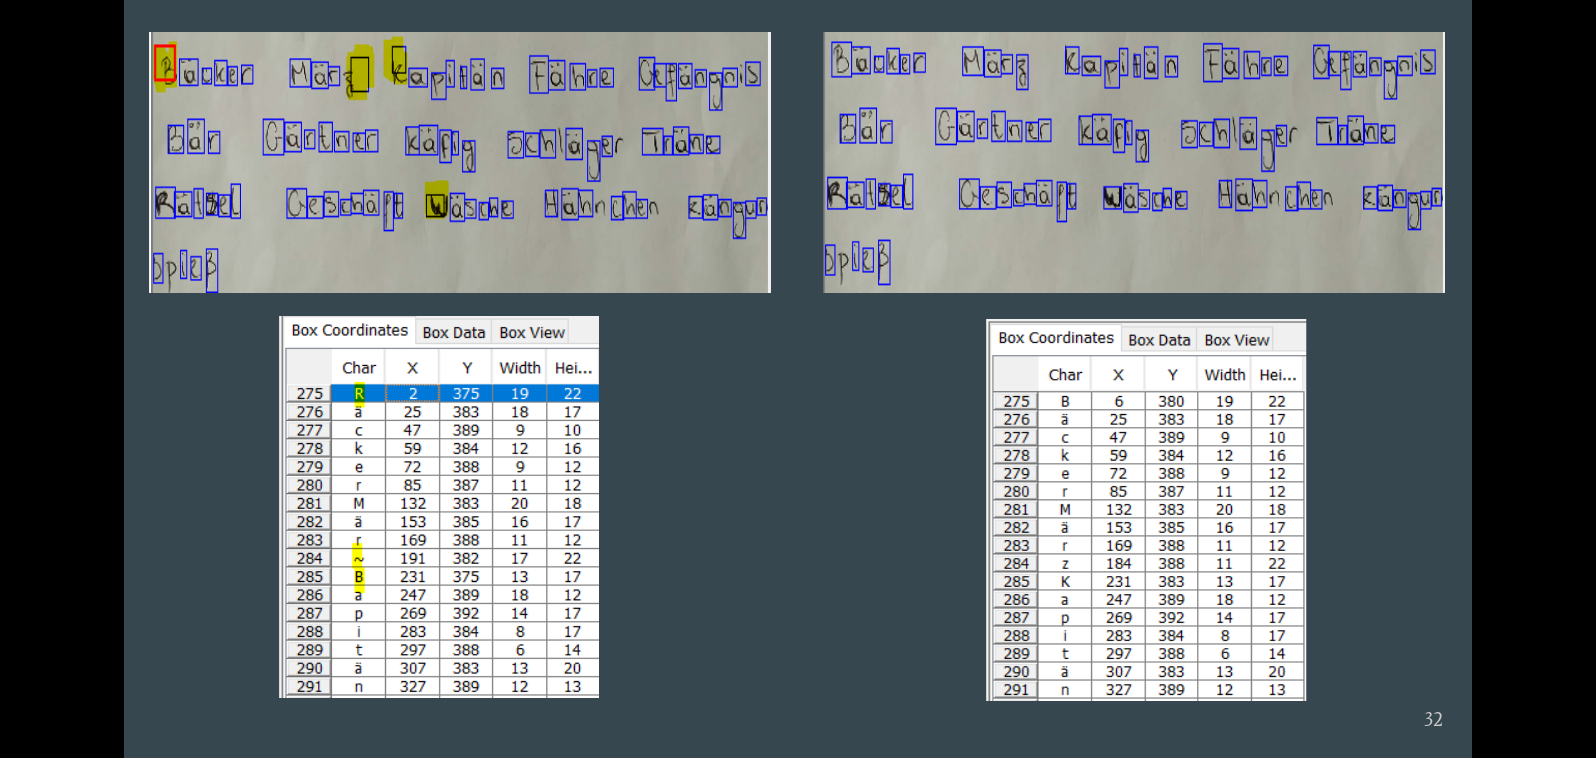
\includegraphics[width=1.0\textwidth]{jtessEditing}
	\caption[Labelling with JTEssboxEditor]{Example of Labelling with JTessBoxEditor} \label{Abb:jtess_editing}
\end{figure}

The picture left shows the characters after they have been predicted and surrounded by boxes using tesseract. 
But some of the predictions are wrong and it is not possible to correctly train the network with such errors. 
Hence the need for labelling.
After labelling with JTessBoxEditor as shown in the picture on the right, the characters are all correct and ready for training. 

\begin{itemize} \bfseries
	\item Training tesseract-ocr on SWTP-AI dataset 
\end{itemize}
The lifecycle from the labelling up to the obtain of the ready model (also called font) will be explained using the figure(\ref{Abb:tess_training}):
For better understanding, the example is done for only one word.

\begin{figure}[htb]
	\centering
	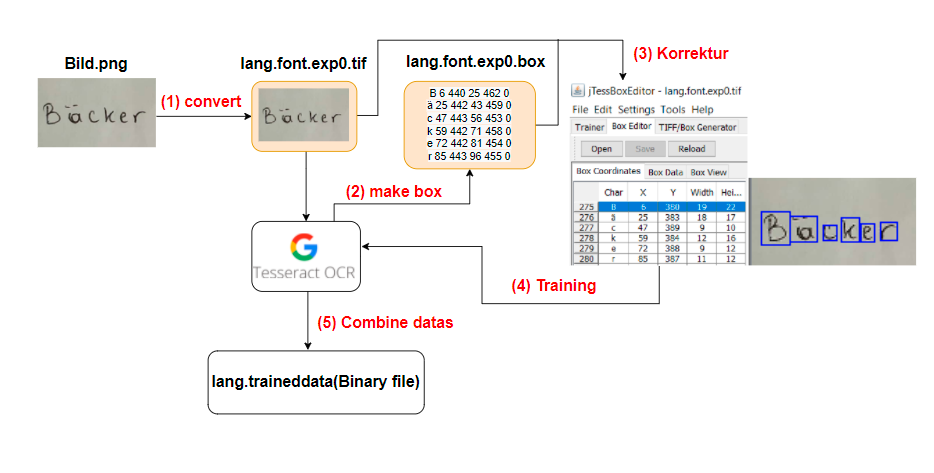
\includegraphics[scale=0.8]{tesseract_training}
	\caption[From writting to trained data File]{Process to get a ready model for training(.traineddata file)} \label{Abb:tess_training}
\end{figure}

The case treated here is to build a model using tesseract which can recognizse the word "Backer". 
tesseract does not necessarily need an image preprocessing.

\noindent
It is firstly important to clarify some concepts like (\cite{[10]}): 
\begin{itemize}
    \item \emph{lang}: is the font language
    \item \emph{font}: is the name of the font
    \item \emph{exp0}: used to tag the the box name used. 
	\item The "exp" varies from exp0 to expn, depending on how many files is used fot the training.
\end{itemize}
The word is firstly written per hand and converted to a .tif format so that, tesseract can be able to use it. 
The conversion is done with the \emph{IMageMagick} tool. The file resulting has the name \emph{lag.font.exp0.tif}:
this is a standard naming convention
Afterwards the .tif format is sent to tesseract and boxes are made as well as each characters predicted. 
The .tif file and the .box files obtained from tesseract are saved in the same folder. 
It is required to save both in the same folder for JTessBoxEditor to recognize them by their names. 
Once in the Editor, the errors are corrected and box coordinates are also correctly adjusted. 
The changes are saved and the two files are sent back to tesseract for the training. 
And after the training all resulting files are combined and the output is a binary file ready  for the prediction process. 
All fonts have the extension \emph{.traineddata}.   
This is generally how the training works.  

\newpage


